% Geometría adaptada de RE_C10: tapas, arcos ocultos y cilindros contiguos.
% Las superficies son esquemáticas; no representan inclusiones de espacios.
\newcommand{\cXVIIItapaDerecha}[3]{%
  \draw[dashed] (#1,#3) arc[start angle=90,end angle=270,
    x radius=#2,y radius=#3];
  \draw (#1,#3) arc[start angle=90,end angle=-90,
    x radius=#2,y radius=#3];}
\newcommand{\cXVIIItapaIzquierda}[4]{%
  \pgfmathsetmacro{\anguloOculto}{asin(#4/#3)}
  \draw (#1,#3) arc[start angle=90,end angle={180-\anguloOculto},
    x radius=#2,y radius=#3];
  \draw[dashed] ({#1-#2*cos(\anguloOculto)},#4)
    arc[start angle={180-\anguloOculto},end angle={180+\anguloOculto},
    x radius=#2,y radius=#3];
  \draw ({#1-#2*cos(\anguloOculto)},{-#4})
    arc[start angle={180+\anguloOculto},end angle=450,
    x radius=#2,y radius=#3];}
% Cono de eje horizontal: vértice a la izquierda y base elíptica a la derecha.
\newcommand{\cXVIIIcono}[3]{%
  \draw (-#1,0)--(0,#3) (-#1,0)--(0,-#3);
  \cXVIIItapaDerecha{0}{#2}{#3}}
% El parámetro 1 añade el cono inicial; 0 deja la tapa visible.
\newcommand{\cXVIIItubo}[1]{%
  \draw (0,.32)--(1.5,.32) (0,-.32)--(1.5,-.32);
  \ifnum#1=1 \cXVIIIcono{1.05}{.10}{.32}
  \else \draw (0,0) ellipse[x radius=.10,y radius=.32];\fi
  \cXVIIItapaDerecha{1.5}{.10}{.32}
  \draw (1.5,.60)--(3.3,.60) (1.5,-.60)--(3.3,-.60);
  \cXVIIItapaIzquierda{1.5}{.16}{.60}{.32}
  \cXVIIItapaDerecha{3.3}{.16}{.60}
  \draw (3.3,.90)--(5.1,.90) (3.3,-.90)--(5.1,-.90);
  \cXVIIItapaIzquierda{3.3}{.23}{.90}{.60}
  \draw[dotted] (5.1,.90)--(5.8,.90) (5.1,-.90)--(5.8,-.90);}

\newcommand{\cXVIIIsuspension}{%
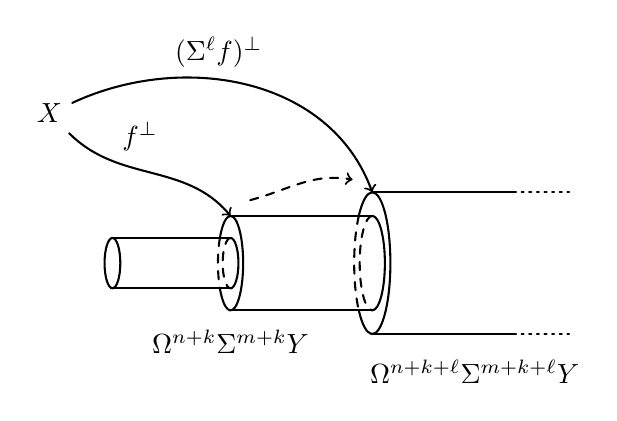
\begin{tikzpicture}[x=1cm,y=1cm,line width=.75pt,line cap=round,
                    line join=round,baseline=(current bounding box.center)]
  \cXVIIItubo{0}
  \node (x) at (-.8,1.9) {$X$};
  \draw[->] (x) to[out=-45,in=130] (1.5,.60);
  \node at (.35,1.61) {$f^\perp$};
  \draw[->] (x) to[out=25,in=110] (3.3,.90);
  \node at (1.35,2.68) {$(\Sigma^\ell f)^\perp$};
  \draw[->,dashed] (1.75,.80) to[out=15,in=170] (3.05,1.06);
  \node[below] at (1.5,-.72) {$\Omega^{n+k}\Sigma^{m+k}Y$};
  \node[below] at (4.6,-1.10) {$\Omega^{n+k+\ell}\Sigma^{m+k+\ell}Y$};
\end{tikzpicture}}

\newcommand{\cXVIIIdoble}{%
\begin{tikzpicture}[x=.80cm,y=.80cm,line width=.75pt,line cap=round,
                    line join=round,baseline=(current bounding box.center)]
  \begin{scope}[shift={(-6.8,0)},scale=.65]
    \cXVIIItubo{0}
    \draw[rojoDiagramaCIMAT] (0,0) ellipse[x radius=.10,y radius=.32];
    \node at (2.4,1.6) {$(RB)_j$};
  \end{scope}
  % Cilindro exterior: sus generatrices rojas conectan las dos etapas.
  \draw[rojoDiagramaCIMAT,->] (.05,1.7)--(.65,-1.7);
  \draw[rojoDiagramaCIMAT,->] (5.1,1.7)--(5.7,-1.7);
  \begin{scope}[shift={(0,1.7)}]
    \fill[yellow!20] (0,-.32)--(1.5,-.32)--(1.5,-.60)
      --(3.3,-.60)--(3.3,-.90)--(5.1,-.90)--(5.1,.90)
      --(3.3,.90)--(3.3,.60)--(1.5,.60)--(1.5,.32)--(0,.32)--cycle;
    \cXVIIItubo{0}
  \end{scope}
  \begin{scope}[shift={(.6,-1.7)}]\cXVIIItubo{0}\end{scope}
  \draw[->] (-6.8,.23) to[out=80,in=180] (-.15,1.7);
  \node at (-3.1,2.29) {$k'_j$};
  \draw[->] (-5.8,-.42) to[out=-60,in=180] (.43,-1.7);
  \node at (-2.8,-2.37) {$\Omega k'_{j+1}$};
  \node at (2.8,3.05) {$(RRC)_j$};
  \node[right] at (6,1.7) {$(RC)_j$};
  \node[right] at (6.6,-1.7) {$\Omega(RC)_{j+1}$};
  \node at (3.2,-3.15) {$\vdots$};
\end{tikzpicture}}

\newcommand{\cXVIIIconos}{%
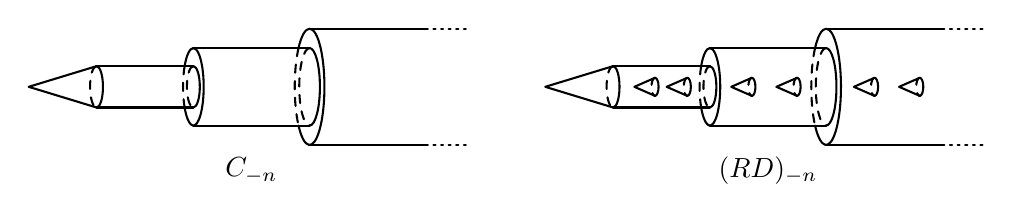
\begin{tikzpicture}[x=.82cm,y=.82cm,line width=.75pt,line cap=round,
                    line join=round,baseline=(current bounding box.center)]
  \cXVIIItubo{1}
  \node at (2.4,-1.30) {$C_{-n}$};
  \begin{scope}[shift={(8,0)}]
    \cXVIIItubo{1}
    % Conos en el interior de cada cilindro, sin cortar las tapas de unión.
    \foreach \x in {.65,1.15,2.15,2.85,4.05,4.75}{
      \begin{scope}[shift={(\x,0)}]
        \cXVIIIcono{.32}{.055}{.14}
      \end{scope}}
    \node at (2.4,-1.30) {$(RD)_{-n}$};
  \end{scope}
\end{tikzpicture}}
